\documentclass[11pt]{article}

%\oddsidemargin=-0.25in				% Left margin minus 1 inch.
%\evensidemargin=-0.25in				% Same for even-numbered pages.
%\textwidth=7in				% Text width (8.5in - margins).
%\topmargin=-0.5in					% Top margin minus 1 inch.
%\headsep=0.2in					% Distance from header to body.
%\textheight=9.25in					% Body height (incl. footnotes)
%\skip\footins=4ex				% Space above first footnote.
%\hbadness=10000					% No "underfull hbox" messages.


\oddsidemargin=-0in				% Left margin minus 1 inch.
\evensidemargin=0in				% Same for even-numbered pages.
\textwidth=6.5in				% Text width (8.5in - margins).
\topmargin=-0.75in					% Top margin minus 1 inch.
\headsep=0.2in					% Distance from header to body.
\textheight=9.5in					% Body height (incl. footnotes)
\skip\footins=4ex				% Space above first footnote.
\hbadness=10000					% No "underfull hbox" messages.

\linespread{1}

\usepackage{amsmath}
\usepackage{mathrsfs}
\usepackage{amsfonts}
%\usepackage{graphicx}
\usepackage{slashed}
\usepackage{cancel}
\usepackage{hyperref}
\usepackage{xcolor}
\usepackage{url}



\hypersetup{linktoc=page}

 \usepackage{feynmp}
 \usepackage[pdftex]{graphicx}
 \usepackage{subfig}
 \DeclareGraphicsRule{*}{mps}{*}{} 

\graphicspath{{Figures/}}

\numberwithin{equation}{section}
%\numberwithin{equation}{subsection}


\newcommand{\p}[1]{\paragraph{#1}}
\newcommand{\hv}{\hspace{2.5cm} \vspace{0.3cm}}
\newcommand{\vs}{\vspace{0.3cm}}
\newcommand{\nin}{\noindent}
\newcommand{\mcal}[1]{\mathcal{#1}}
\newcommand{\da}{{\dot{a}}}
\newcommand{\db}{\dot{b}}
\newcommand{\dc}{\dot{c}}
\newcommand{\dd}{\dot{d}}
\newcommand{\la}{\langle}
\newcommand{\ra}{\rangle}
\newcommand{\wh}{\widehat}
\newcommand{\wt}{\widetilde}
\newcommand{\lam}{\lambda}
\newcommand{\Lam}[2]{\Lambda^{#1}_{\ #2}}
\newcommand{\tlam}{\wt{\lambda}}
\newcommand{\del}{\partial}
\newcommand{\sigx}{\sigma_x}
\newcommand{\sigy}{\sigma_y}
\newcommand{\sigz}{\sigma_z}
\newcommand{\oft}{\left(t\right)}
\newcommand{\rarr}{\rightarrow}
\newcommand{\larr}{\leftarrow}
\newcommand{\tdot}{\cdot \cdot \cdot}
\newcommand{\diff}[1]{ \frac{d #1}{ds} }
\newcommand{\pdiff}[2]{ \frac{ \partial #1 }{ \partial #2 }}
\newcommand{\ket}[1] { |  #1 \ra }
\newcommand{\bra}[1] { \la #1 | }
\newcommand{\braket}[3] { \la #1 | #2 | #3 ] }
\newcommand{\sumlim}[3] { \sum\limits_{#1 = #2}^{#3} }
\newcommand{\prodlim}[3] { \prod\limits_{#1 = #2}^{#3} }
\newcommand{\om} {\omega}
\newcommand{\Om}{\Omega}
\newcommand{\xx}[1] {\cancel{#1}}

\newcommand{\tit} {\textit}
\newcommand{\gam} {\gamma}
\newcommand{\Gam}[2] {\Gamma^{#1}_{#2}}




\begin{document}

\title{\textbf{Microwave Impedance Microscope for Hybrid Superconductor-Semiconductor Devices}}
\author{\\Seongwoo Oh}
\date{11/7/2015}
\maketitle

%\newpage
\tableofcontents
%\newpage

\section{Introduction}
\hspace{\parindent}
In recent years, semiconductor quantum dot technology has made a tremendous amount of progress in the quantum technology race. A large part of such progress has come from the Petta lab in the form of designing an overlapping gate structure and integrating a superconducting resonator in silicon quantum dot devices.  Such innovations rendered semiconductor quantum dot as a serious contender in relation to what used to be the two most competitive physical relizations of quantum computer: trapped ion, superconducting qubit. However, there are several pressing issues that currently limit the progress in this race for semiconductor quantum dot technology.  Little is understood about the valley-states and charge noise.  
Therefore, not a clear path toward tackling these issues has been proposed.  The main reason for the lack of clear vision toward resolving the issues is that there has not bee a probing tool appropriate for addressing them.  In this pre-thesis, we propose a scanning probe, which would not only help shed light on the issues mentioned above in the context of semiconductor qubit, but also enable progress in topological quit and fundamental research.  


\section{Design Overview}
\hspace{\parindent}
Our proposal is based on several elements derived from existing designs.  One of such designs is the conventional tuning fork based AFM (atomic force microscopy) design, as shwon in figure 1 below \cite{zxsafm}. 

\begin{figure}
	\centering
	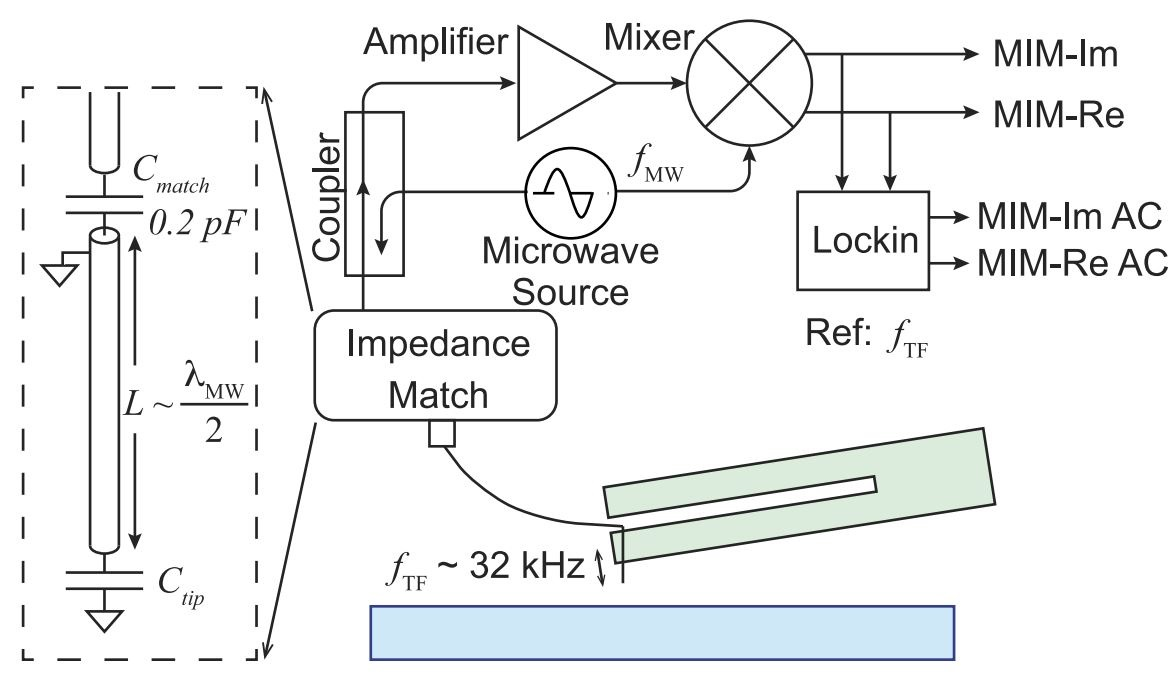
\includegraphics[scale=0.4] {mimcircuit.jpg}
	\caption{conventional microwave impedance microscope circuitry }
	\label{mimcircuit}
\end{figure}

The standard AFM technique is used to map the surface morphology of a sample.  While topograhic information is acquired, microwave signal is sent and interacts with the sample at the tip-sample junction. The reflected signal (S11 parameter) offers rich information about the permitivity and conductivity of the sample under study \cite{kejilai}.  For some of the experiments that we have in mind, the scanning probe that we need to build will also have STM measurement capability.  This point will be discussed in greater detail in a later section.  The quartz crystal tuning fork is another crucial aspect of the project and will be discussed further.\\

Another existing design idea that our research will build on is incorporating a superconducting resonator in the scanning probe \cite{graaf}.   In reference 3, the group designed a fractal resonator for the purpose of having a resonator in the GHz regime while keeping the resonator light and compact enough to be glued to the tip of a tuning fork without destroying the mechanical resonance of the tuning fork (around 32KHz).  A superconducting resonator of the usual meander design would result in too large and heavy a size to be glued to the tuning fork. \\

For the main body of our scanning probe design proposal, we have used the design most commonly used in the STM/AFM community: ``the Pan-walker'' design \cite{pan}.  \\

Petta lab routinely patterns superconducting resonators as part of overlapping gate structure quantum dot devices.  Therefore, patterning a resonator in the GHz regime was not seen as a challenge.  The only difference introduced in this project is that the resonator would have to be patterend on a quartz substrate, as tuning forks are made of quartz crystal.  Hanger resonators are often patterend when trying out a new wafer.  Since quartz wafers are never used in Petta lab, hanger resonatros were patterend, and transmission spectrum was analyzed for quality factors and resonance frequencies.  The measured quality factors and resonance frequencies are compared to design quality factors and resonance frequencies. \\

Earlier, a superconducting cavity patterened on a chip glued to a quartz tuning fork was shown as part of our design inspiration.  Similarily, a metalic tip, prepared through chemical etching, is glued to a tuning fork in the case of conventional MIM design. However, manually gluing a probe tip results in too much varability in producing probe heads.  \\

One of the big challenges in our design proposal is to seamlessly integrate a superconducting resonator into the tuning fork, which is the crux of the microscope head.  Rather than fabricating a resonator and gluing it to a commercial tuning fork, integrating a superconducting resonator into the tuning fork fabrication recipe would remove a great deal of uncertainty in characteristics of tuning forks and superconducting resonators.  If a resonator on a separate chip needs to be manually glued to a tuning fork, the mechanical resonance frequency of the tuning fork after gluing could vary greatly.  It simply is not feasible to make this process perfectly repeatable.  We are going to outline how we plan to tackle this problem in a later section.   



\begin{figure}%
    \centering
    \subfloat{{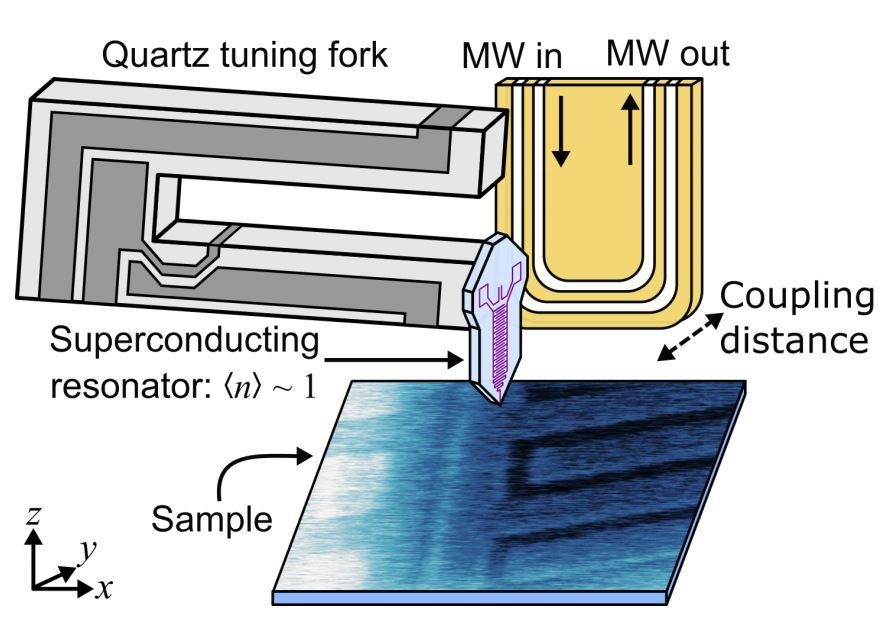
\includegraphics[width=6cm]{degraaf} }}%
    \qquad
    \subfloat{{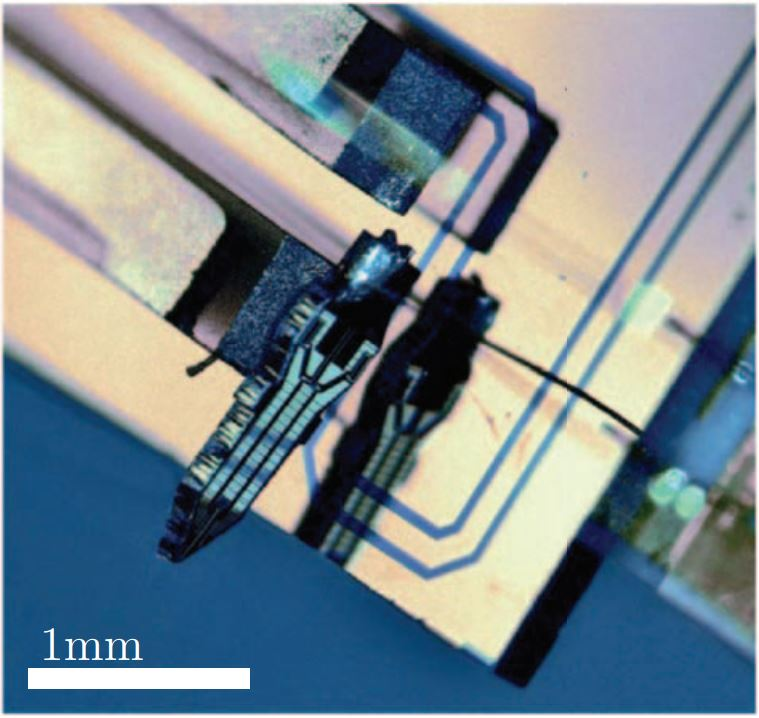
\includegraphics[width=4.8cm]{sdegraaf} }}%
    \caption{schematic and real images of resonator on quartz tuning fork}%
    \label{fig:example}%
\end{figure}







\section{Brief Overview of Pan Walker}



\begin{figure}%
    \centering
    \subfloat{{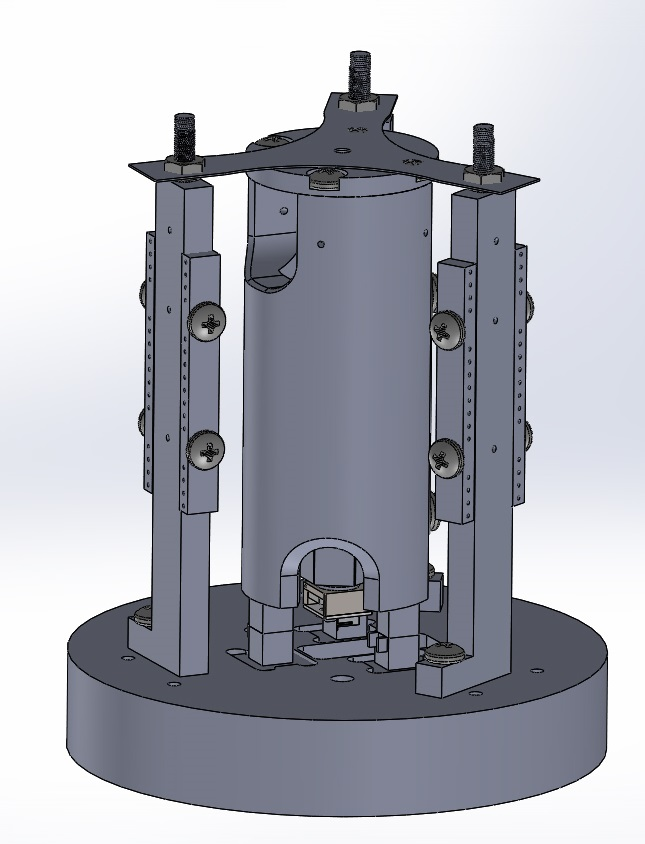
\includegraphics[width=6cm]{headtop} }}%
    \qquad
    \subfloat{{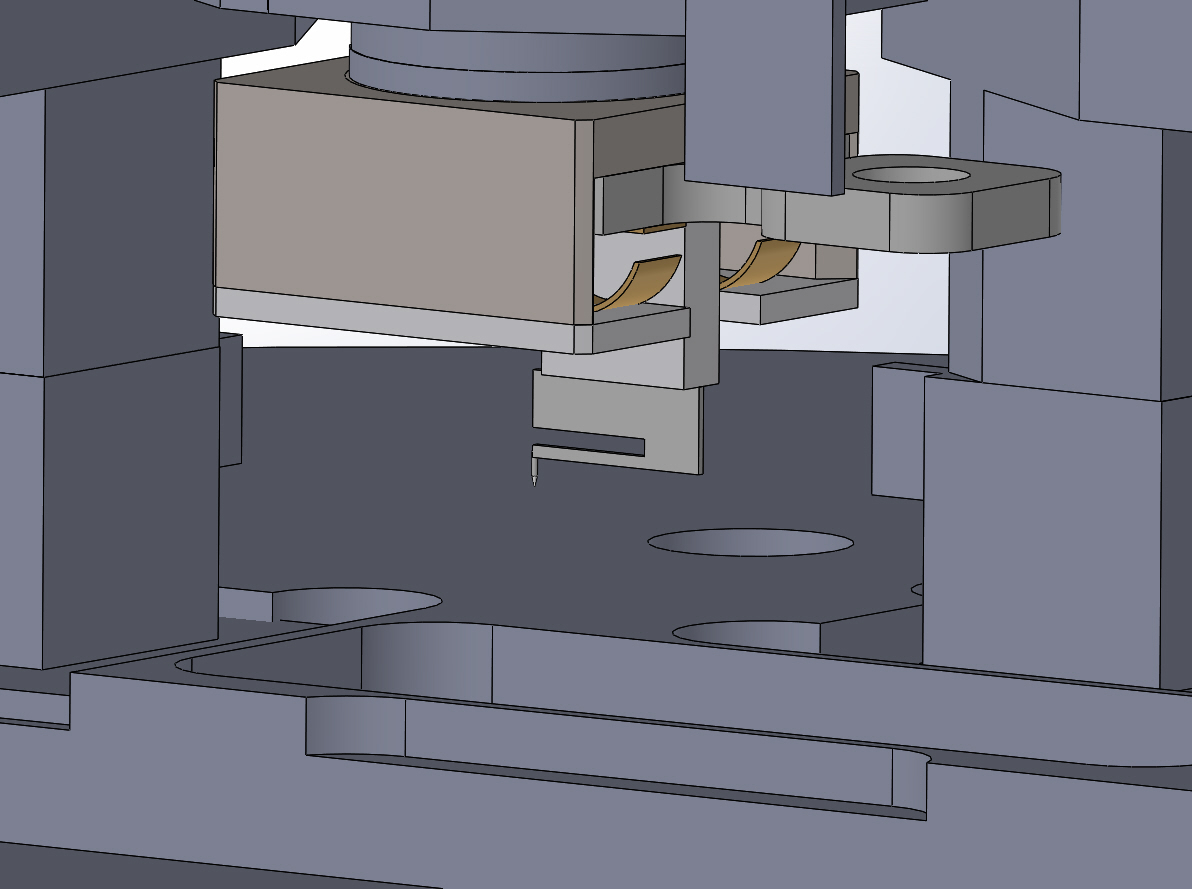
\includegraphics[width=4.8cm]{closeup} }}%
    \caption{rendering of Pan-walker scanning probe with close-up of probe head}%
    \label{fig:example}%
\end{figure}

\hspace{\parindent}
Figure 3 is a rendering of the Pan-walker type microscope in Solidworks. The scope is expected to be housed in a BlueFors XLD series dry fridge. With a standard vacuum can for the fridge not having an optical view port, there was no need to design a radiation shiled for the scope. The tuning fork part of the scanning probe head is designed to be easily removable.  At the center of the elongated structure resides a tube piezo, the dimensinos of which determines the scanning range of the scanning probe. The tube piezo dimensions are chosen with a target scanning range of 10um in mind.   The tube piezos were ordered from EBL piezoelectric precision based on the following equation \cite{EBL}.  



\begin{equation}
\Delta x, \Delta y = \frac{0.9 d_{31} V L^{2}}{d_m t}
\end{equation}  \\

,where $d_{31}$, $V$, $L$, $d_m$, and $t$ are a temperature dependent coefficient, voltage applied to two opposite quadrants of the piezo tube, length, average of the outer and inner diameters, and thickness of the piezo tube respectively. The length of the piezo tube is chosen such that the scanning range is around \( 10\ \mu \)m in both $x$ and $y$ directions.\\

\begin{figure}
	\centering
	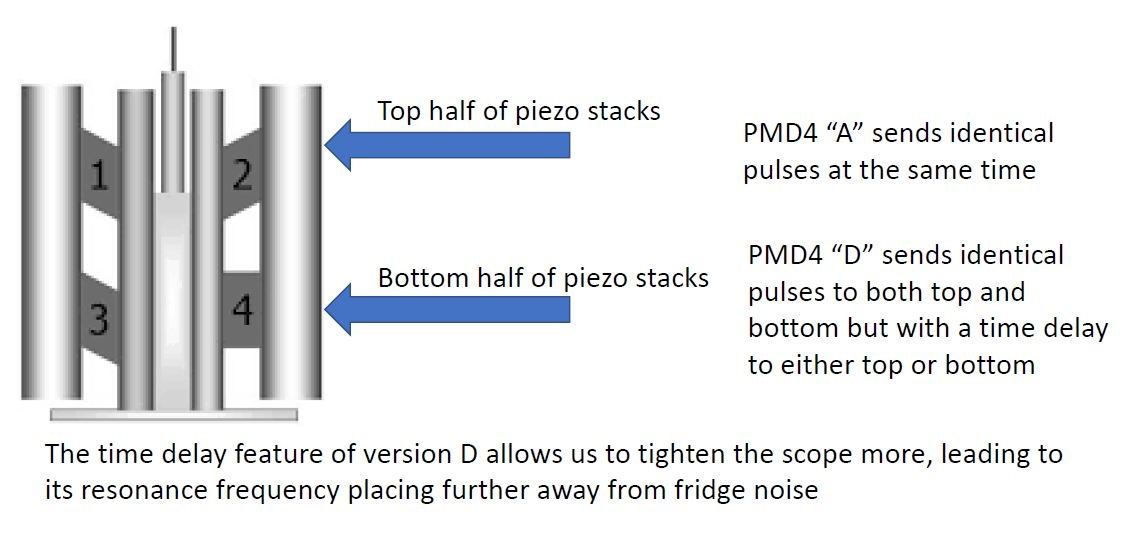
\includegraphics[scale=0.4] {pmd4dimage.jpg}
	\caption{schematic explaining operating principle of PMD4D}
	\label{pmd4image}
\end{figure}

The piezo and scanning probe controllers to operate the microscope are products from Nanonis.  Since the Nanonis scanning probe suite is staple in the STM/AFM community , instead of going into detail about the electronic equipment, I will point out one subtlety to consider when choosing the right piezo driver, in the context of piezo actuation.  Nanonis offers 4 different versions of PMD4 piezo driver. However, this is not mentioned in their brochure, and version A is the default choice.  Version D is advantageous . Version A sends pulses to all piezo legs of the Pan walker at the same time, whereas version D sends pulses to the top half of the piezo legs at time T and the bottom half at T + $\delta$T.  This slight time delay allows the scope to be assembled tighter, leading to the body of the microscope to have a higher mechanical resonance frequency. So, the scope is better decoupled from the fridge's vibration.  Also, version D is reported to be less prone to occasional piezo stoppage at cryogenic temperatures. \\

In the rest of the write-up, we will discuss etching metallic tips, which will be used in the conventional STM/AFM mode for dry fridge vibration noise and Pan-walker characterization, testing superconducting resonators on quartz substrate, acquiring preliminary topographic images under ambient conditions, and designing resonator integrated tuning fork. \\

\section{Tip Etching}
\hspace{\parindent}
In conventional MIM(Microwave Impedance Microscopy), having a sharp metallic tip is crucial, as the sharpness of the probe is the sole factor in determining the spatial resolution of the microscope. Chemical etching is the most commonly accepted way of tip sharpening in the context of scanning probe.  Broadly speaking, a metallic wire, either a W or Pt/Ir wire is dipped into an etchant with a finite voltage bias applied to the etchant and wire.  Etchant concentration, amplitude and cutoff of voltage bias determine the sharpness of the tip. Since stopping the chemical reaction when the tip is at its sharpest is crucial, various feedback circuits have been proposed in the past \cite{tip}. Several feedback methods, including Labview scripting, were tried without much success.  The most promising result was obtained by so-called ``double lamellae dropoff \cite{doublela}.'' \linebreak


\begin{figure}
	\centering
	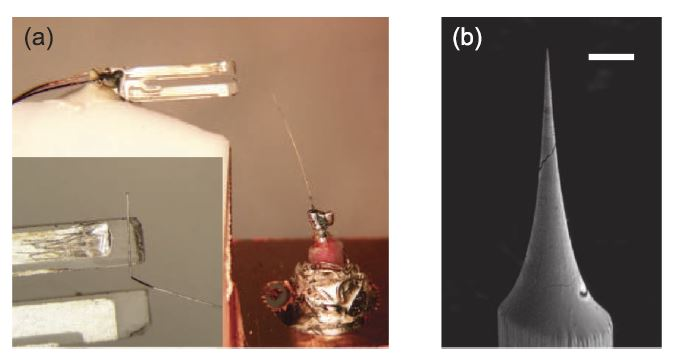
\includegraphics[scale=0.6] {shentip.jpg}
	\caption{example of Pt/Ir tip. Scale bar:\( 10\ \mu \)m}
	\label{shentip}
\end{figure}

As opposed to having an electronic feedback circuit, this method uses gravity as a cutoff switch. The polarity of the voltage bias was chosen such that the upper end of the wire that hangs above the etchant beaker is the sharp end and used as a tip.  \\

\begin{figure}
	\centering
	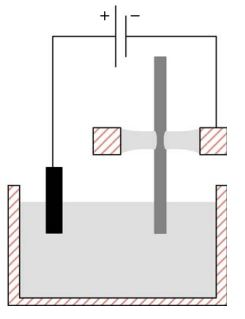
\includegraphics[scale=0.7] {doublelacircuit.jpg}
	\caption{schematic of double lamellae dropoff circuit \cite{doublelacircuit}}
	\label{doublelacircuit}
\end{figure}


Here, we report the etching parameters and present images of a resulting tip.  A Keithley 2400 was used in the constant voltage mode for 5V bias.  The diameters of both W and Pt/Ir wires used are 0.001 inches. 4.5 grams of KOH are dissolved in 40mL of DI water for W, and 1.75 grams of CaCl2 are dissolved in 20mL of DI water to have a molar concentration of 2M (Pt/Ir is often preferred, as Pt is inert to oxidation, albeit much more expensive than W).\\

\begin{figure}%
    \centering
    \subfloat[overview of tip]{{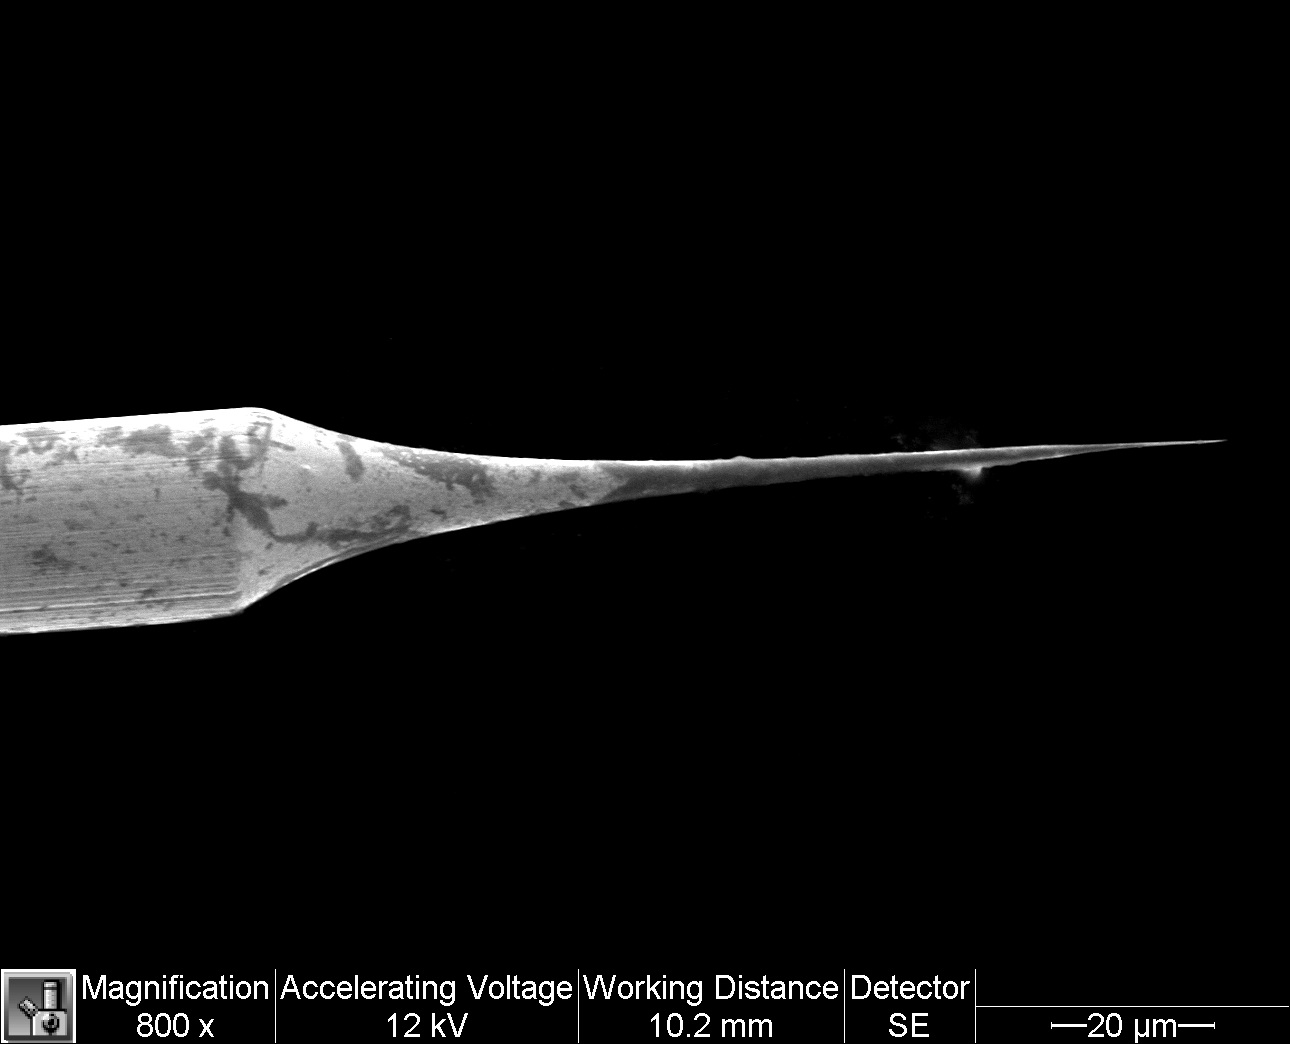
\includegraphics[width=7.5cm]{tipimage} }}%
    \qquad
    \subfloat[close up of near end of tip]{{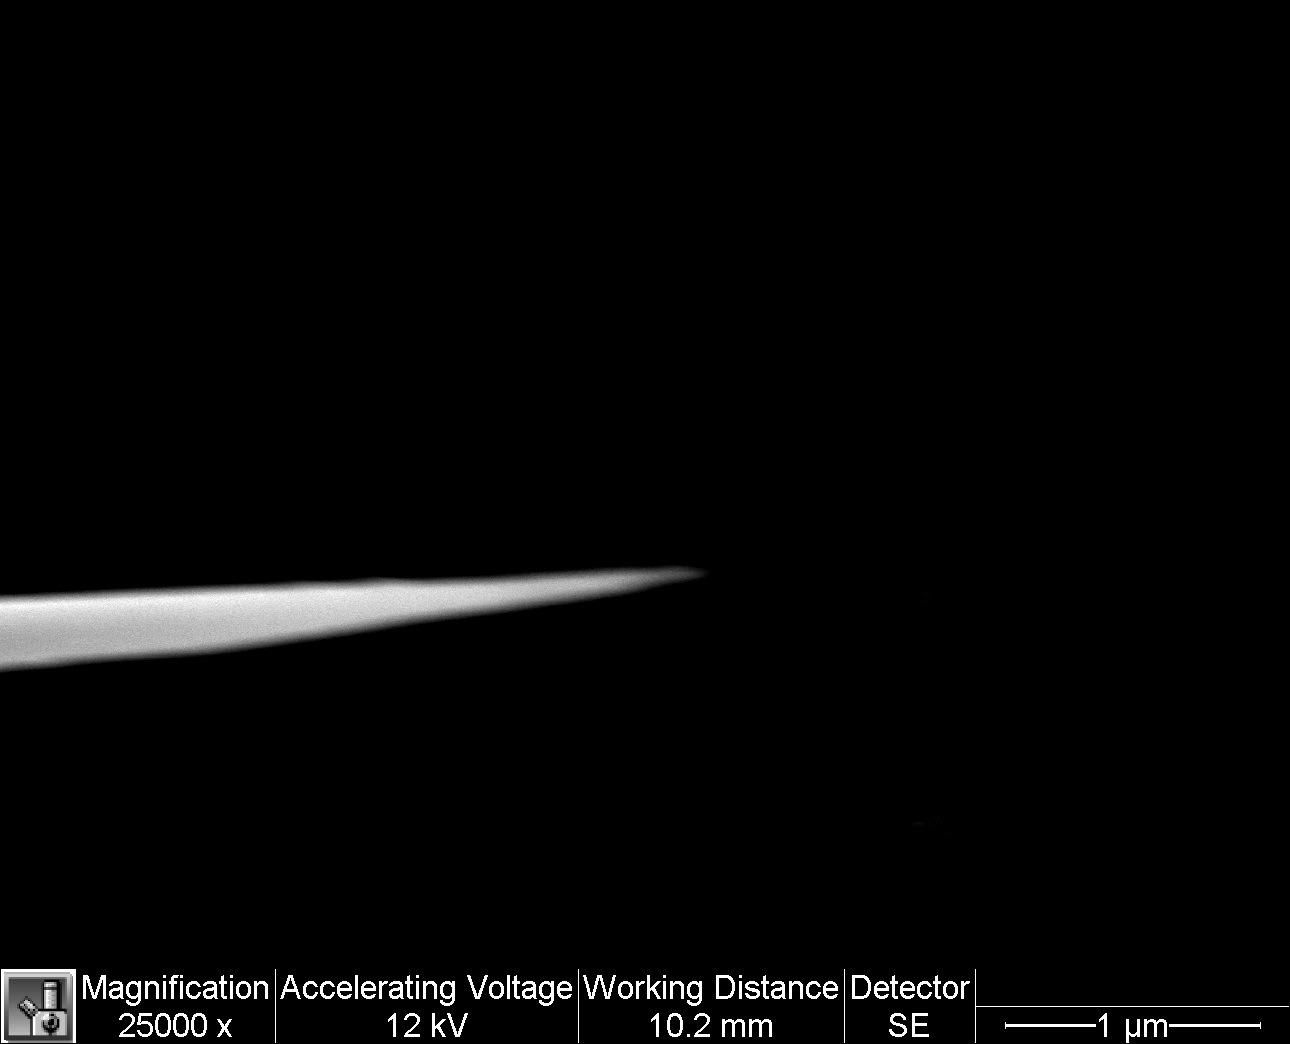
\includegraphics[width=7.5cm]{tipimageclose} }}%
    \caption{SEM images of W tip}%
    \label{fig:example}%
\end{figure}

Figure 7 shows W tips etched following the recipe described above. The images were taken with the SEM (XL30) at the PRISM Imaging and Analysis Center.  In the image on the left, what may appear to be an irregular surface or dirt near the middle of the taper is a surface irregularity of the conductive tape that the tip sits on.  \\

\begin{figure}%
    \centering
    \subfloat[overview of tip]{{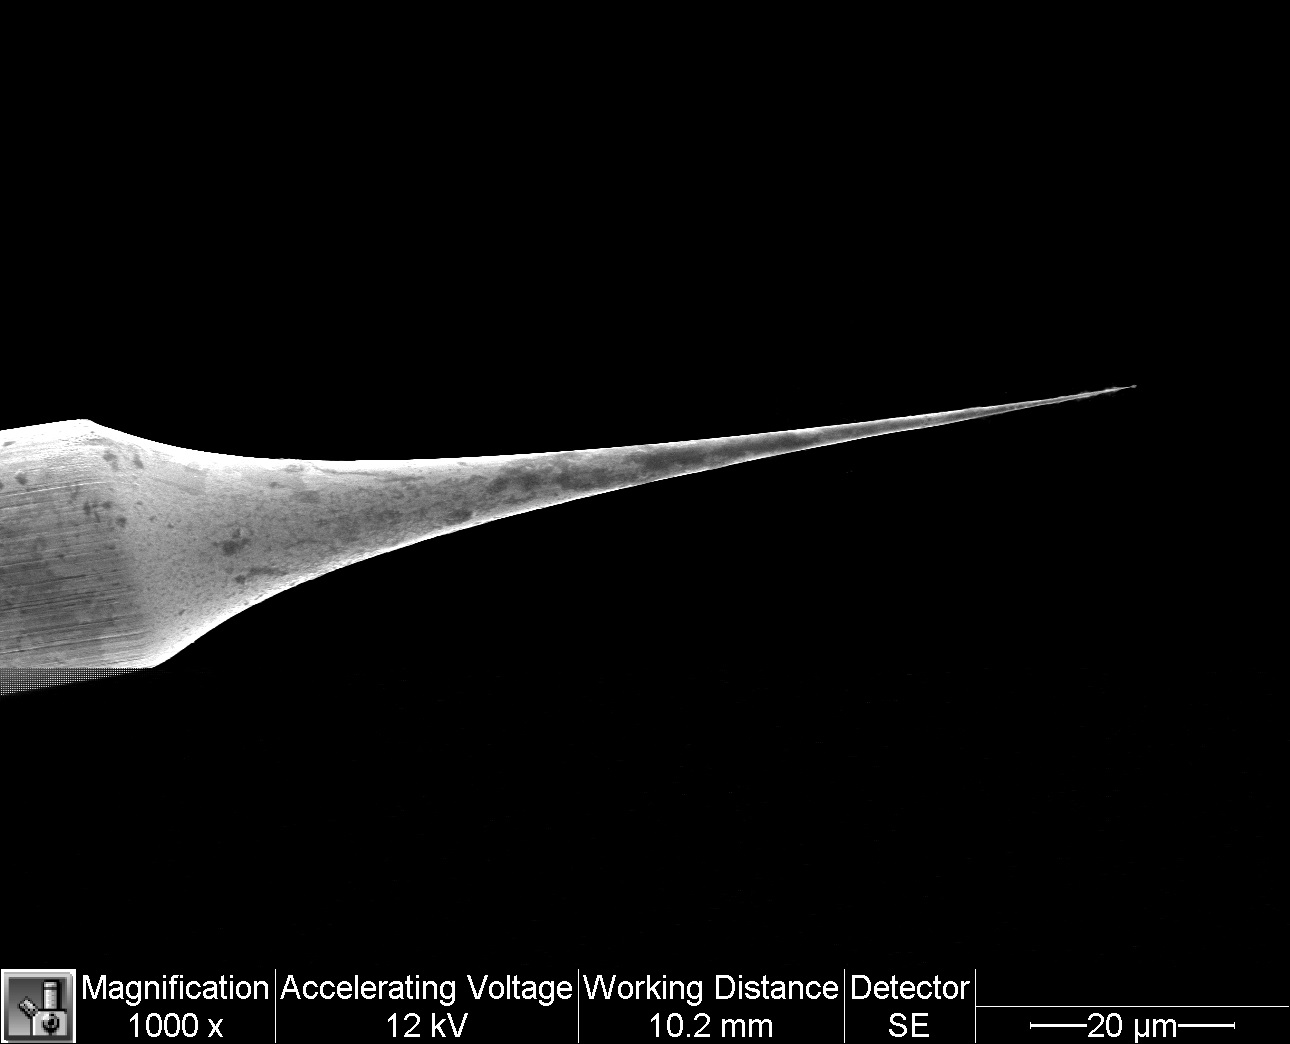
\includegraphics[width=7.5cm]{tipimagebad} }}%
    \qquad
    \subfloat[close up of near end of tip]{{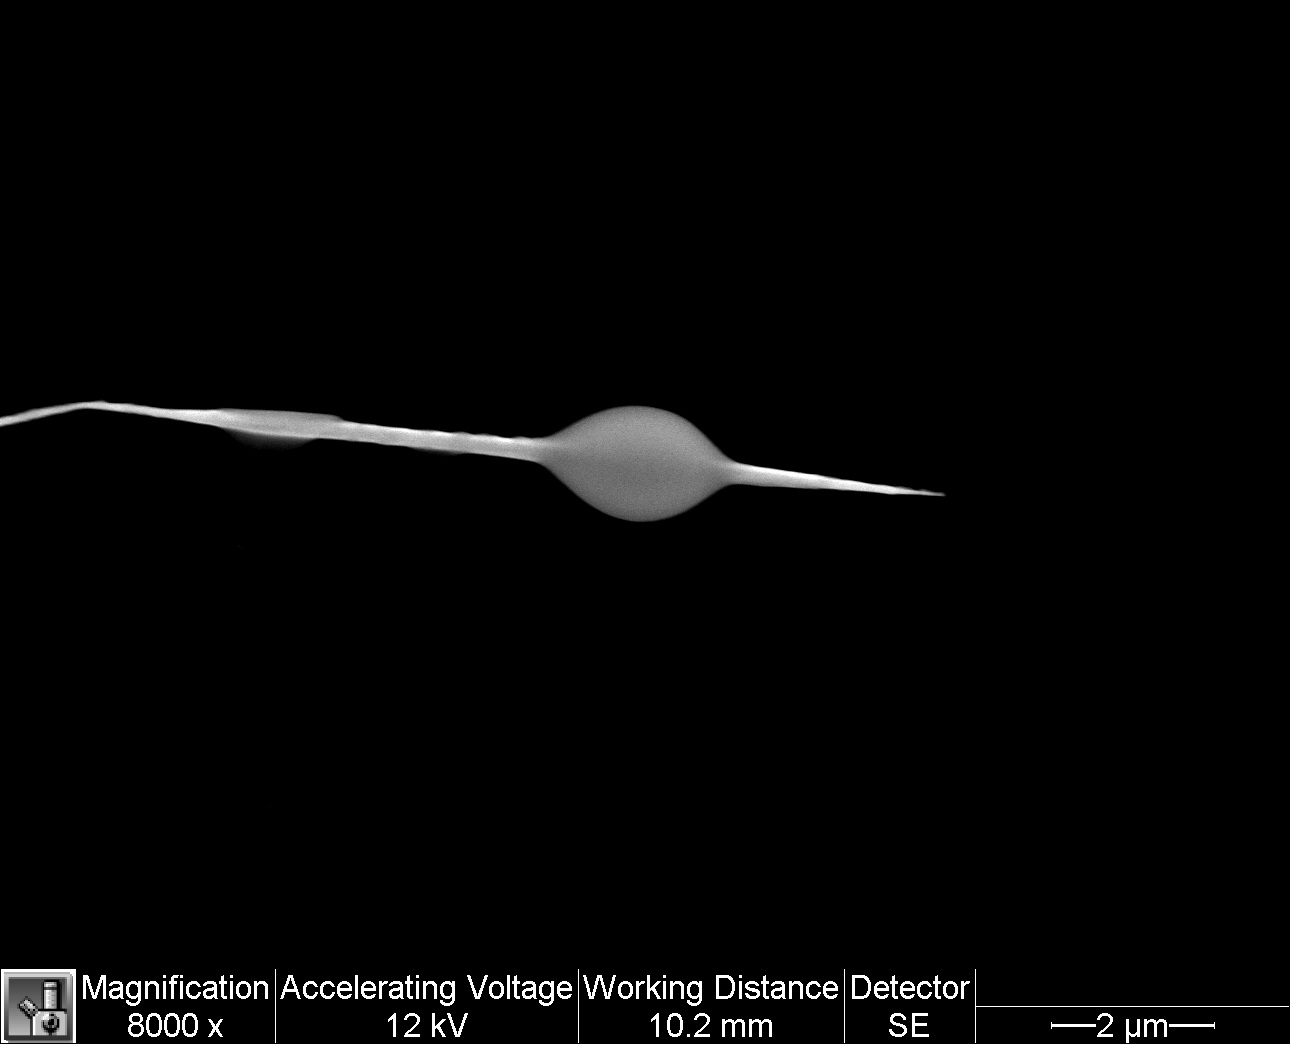
\includegraphics[width=7.5cm]{tipimagebadclose} }}%
    \caption{SEM images of bad W tip}%
    \label{fig:example}%
\end{figure} 

Despite the double lamellae method producing a good tip on a much more consistent basis than other methods, it does occasionally result in less than ideal tip shape, as can be seen in figure 8.  It must be acknowledged that this is impossible to eliminate with absolute certainty, and therefore after each round of tip preparation, one must take preliminary topographic measurement of sample surface morphology to determine whether or not one has a good probe tip. \\

\section{Resonator Design, Fabrication, and Characterization} 

\hspace{\parindent}
Since a superconducting resonator is intended to be integrated into the scanning probe's quartz tuning fork, it is beneficial to study resonator design's compatibility with quartz when the material is used as a substrate.  Due to the simplicity of the design and ease of fabrication, hanger resonators are often patterned, and scattering parameters are measured when testing a new wafer.  For the purpose of testing the suitability of quartz as a substrate, hanger resonators of various quality factors and resonance frequencies are designed, fabricated, and characterized.   \\


\subsection{Resonator Design}

\hspace{\parindent}
Design characteristics of hanger resonators are well understood, as they have been patterend and measured many times on silicon \cite{mazin}. 
In general, it is desirable to select dimensions of resonators in order to have impedance matched.  Most RF instruments have 50\(\ \Omega \) termination, and so resonator dimensions are chosen to give 50\(\ \Omega \) characteristic impedance.  The characteristic impedance of a resonator is a function of relative dielectric constant,\(\ \epsilon_{r} \), track width, gap width, and dielectric thickness.   With the given dimensions and a 500 mm thick quartz substrate, the characteristic impedance comes out to be 83.69 \(\Omega \)  \cite{marsrover}.  \\

\begin{figure}
	\centering
	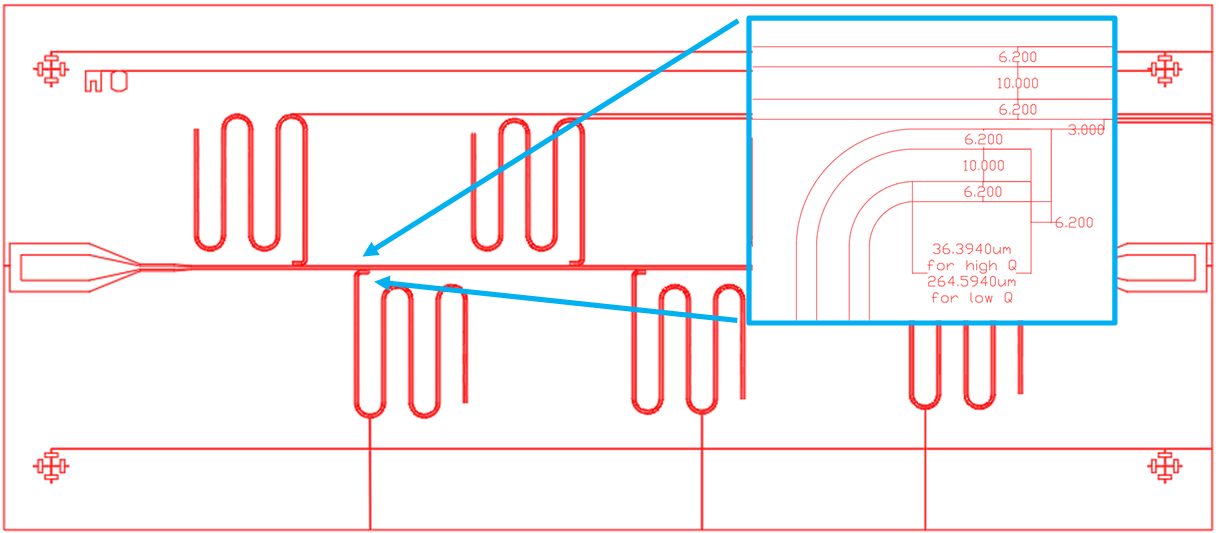
\includegraphics[scale=0.5] {Drawing1}
	\caption{AutoCAD drawing of high Q resonator (inset has dimensions indicated in\(\ \mu \)m )}
	\label{doublelacircuit}
\end{figure}

\begin{figure}
	\centering
	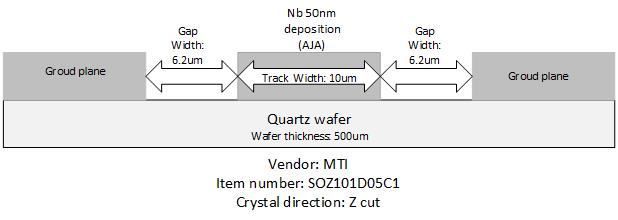
\includegraphics[scale=0.7] {crosssectional}
	\caption{cross sectional view of resonator on quartz substrate}
	\label{crosssectional}
\end{figure}

The dimensions shown in the inset of figure 9 are chosen to give a characteristic impedance of 50\(\ \Omega \) for silicon substrates.  Often, it is desirable to intentionally design a high impedance resonator, as higher impedance leads to larger amplitude for the electric field; one example of this being desirable is when a resonator is coupled to a quantum dot. For this reason, the same dimensions are used for resonators on quartz.  However, the length of the coupling region for the hanger resonators is modified in order to achieve different capacitive coupling strength. The longer the coupling region between the transmission line and the bracket of the hanger resonator, the stronger the capacitive coupling.  Higher capacitive coupling means more energy is leaked, and therefore the quality facotor of the resonator is designed to be lower. In the $S_{21}$ parameter measurement, energy transmission is measured between the two ports of the center line, shown in figure 9.  Near the center line, there are 6 hanger resonators with slightly different lengths.  Those 6 resonators show up in the $S_{21}$ spectrum measurement as 6 dips as energy is leaked into the resonators at their resonance frequencies. \\

With all the dimensions of the resonator and characteristic impedance determined, the only parameter missing to calculate the design quality factors and resonance frequencies is the capacitance between the hanger resonators and the center line.  We use two methods to simulate the capacitance value of the junction between the center line and the hanger resonator.  The first method is to use ``ANSYS Maxwell'' to directly simulate the capacitive coupling.  

\begin{figure}%
    \centering
    \subfloat{{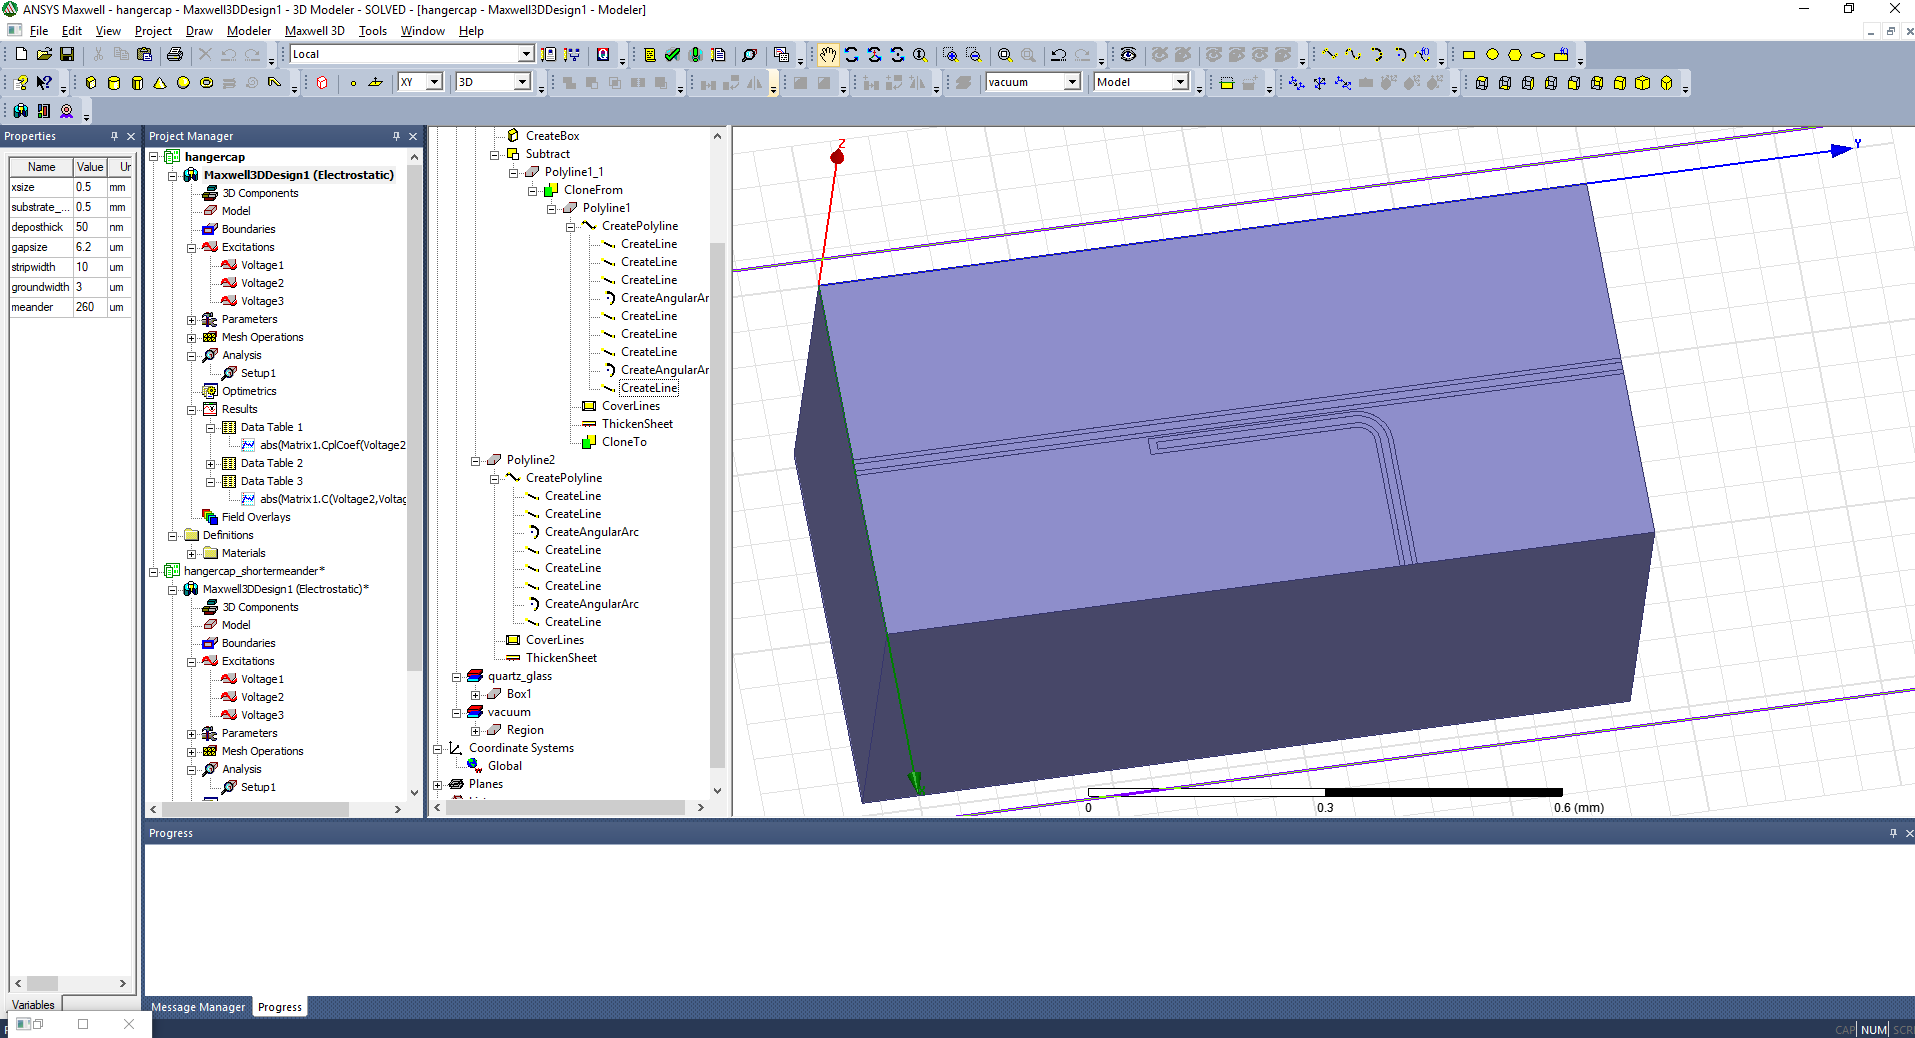
\includegraphics[width=6.7cm]{hangercapmaxwell} }}%
    \qquad
    \subfloat{{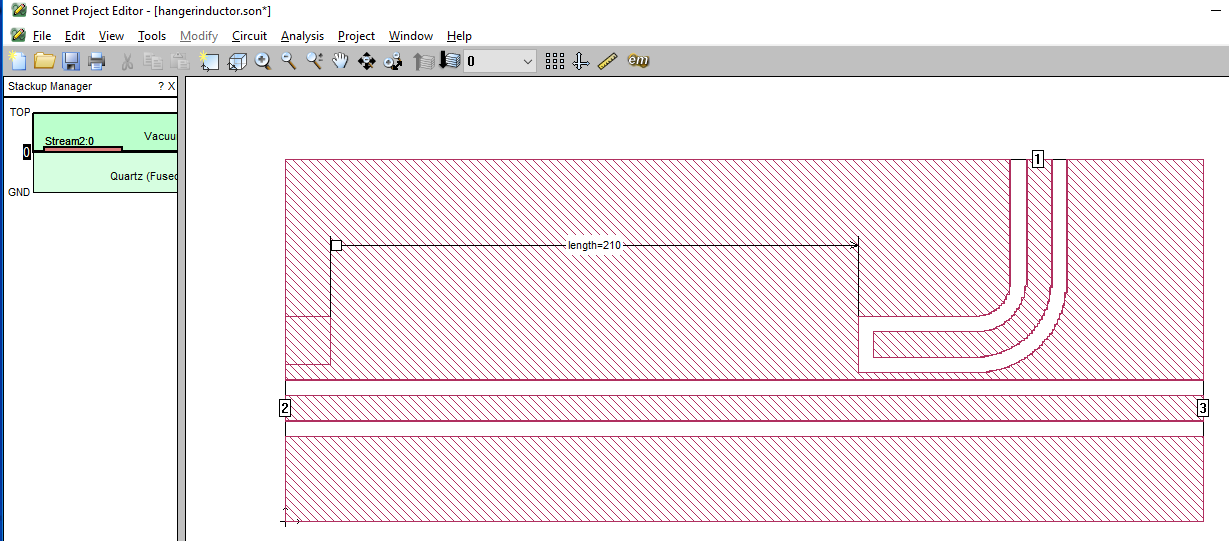
\includegraphics[width=8cm]{sonnet} }}%
    \caption{capacitive junction set up in Maxwell and Sonnet}%
    \label{fig:example}%
\end{figure} 




\bibliographystyle{unsrt}
\bibliography{references}

\end{document}


